\documentclass[12pt]{report}
\usepackage[utf8]{inputenc}


\usepackage{natbib}
\usepackage{graphicx}
\usepackage{xcolor}
\usepackage{amsfonts}
\usepackage{amsmath}
\usepackage{amssymb}
\usepackage{subfig}

\setcounter{secnumdepth}{4}
\renewcommand{\baselinestretch}{1.5}
\DeclareMathOperator*{\argmax}{arg\,max}

\usepackage{fancyhdr}
\bibliographystyle{unsrt}

\pagestyle{fancy}
\fancyhf{}
\rhead{\footnotesize{\textit{What does ESG Data teach us about corporate sustainability?}}}
\lhead{\footnotesize{\textit{Sarah Jallot}}}
\rfoot{Page \thepage}

\begin{document}
\begin{titlepage}
\newcommand{\HRule}{\rule{\linewidth}{0.5mm}}
\begin{figure}[!tbp]
  \centering
  {
\includegraphics[scale=0.1]{hec_logo.png}} 
  \hfill
  {
\includegraphics[scale=0.1]{polytechnique_logo.png}}
\end{figure}
\textcolor{white}{test}\\[0.5cm]
\center
{\large M2 / Data Science for Business X-HEC Major} \\[1cm]
{\large Master Thesis} \\
{\large Academic Year of 2020-2021} \\[1cm]
\HRule \\[0.2cm]
{\large \textbf{What does ESG Data teach us about corporate sustainability? A data-driven case study to support sound investment decisions.}}
\HRule \\[1cm]
{\large Sarah Jallot} \\ 
{\large Under the Supervision of Sylvain Le Corff, Machine Learning \& Statistical Theory Professor at Telecom SudParis and École Polytechnique, ex-CNRS researcher } \\ [1cm]
{\large Public Report} \\ 
\end{titlepage}


\begin{titlepage}
\section*{Acknowledgements}
When I started looking into Sustainable Finance in October 2020, Environment, Society and Governance data for investors to evaluate corporate sustainability was a mystery to me. Over \textbf{60 Sustainable Finance experts} were instrumental in setting the stage for this Master Thesis. Thank you for walking me through the intricacies of this complex topic, from its inception to its current challenges.\newline
\newline
But this report would have been incomplete without its Data Science investigation. A warm thank you to \textbf{Sylvain le Corff}, Statistics and Machine Learning Professor at Telecom SudParis and Institut Polytechnique de Paris, for his close supervision and mentoring during this Master Thesis.\newline  
Thank you to \textbf{Solenne Niedercorn} and \textbf{Mathias Abramovicz} for their unfailing support in discovering the Sustainable Finance Market and ESG during HEC Paris's Start-Up Launchpad - always challenging our team to be more practical and execution-oriented.\newline 
A special thank you to \textbf{Etienne Vincent} and \textbf{Lan-Anh Tran} for their precious mentoring during the portfolio management \textit{2021 Natixis Investment Managers Graduate Challenge} in implementing a robust Quant and ESG Strategy, and to  \textbf{Brice Royer} for his sharp insights on the market's legal aspects, especially within the European Union.
\newline
\newline
Last but not least, thank you to my Start Up Launchpad teammates \textbf{Guillaume Le Fur}, \textbf{Mathieu Joubrel} and \textbf{Anna Logacheva} for delving deep down into the murky waters of ESG Finance together.
\end{titlepage}
\begin{titlepage}
\section*{Statement of Originality}
I confirm that the enclosed material is all my own work. I have not copied or based my work on samples or exemplars to which I have had access. Any work taken from another source has been appropriately referenced and acknowledged.
\end{titlepage}

\begin{titlepage}
\section*{Executive Summary}
Sustainable Investing is \textbf{gaining momentum} in a context where mindsets towards \textbf{ESG\footnote{Environment, Society, Governance.} investing}, that is to say the integration of sustainability considerations into investment processes, have \textbf{drastically evolved}.\newline \newline
ESG used to be an \textbf{ethical box to check}. It is now \textbf{impossible to miss}. Investors are facing dire \textbf{pressure} from across the board to \textbf{integrate sustainability} at the \textbf{core} of their investment process. From \textbf{regulators}, with the European Union spearheading ESG \textbf{standardisation} initiatives. From \textbf{clients}, who want sustainable portfolios but are (rightly) confused by 'ESG' products. And by \textbf{civil society} at last, with rising concerns about \textbf{Climate Change} impact on business operations.\newline
But the ESG industry cruelly lacks \textbf{quality} \& \textbf{standardised data}. No ESG Analysis frameworks are exploitable at scale for investors and other participants. To illustrate this expert interview finding, we decide to investigate to what extent the new Sustainable Finance Disclosure Regulation (SFDR) can be used as an ESG Analysis framework. We use the 32 mandatory Environmental, Social and Governance indicators that it requires to disclose at portfolio level to \textbf{predict ESG Performance} for for over \textbf{2,800 companies}, using notations by \textbf{two different notation agencies} as targets.\newline
This Master Thesis aims to help make \textbf{sustainability-related corporate data} actionable for investors in their due diligence process. It goes as follows. We start by laying out the current \textbf{business and regulatory context} of ESG Data and defining the challenges around its \textbf{collection, interpretation, and integration} to stock investment decisions. We then use \textbf{notation agency ESG data} and \textbf{Machine Learning} to build our understanding of companies' ESG Performance, based on \textbf{Sustainable Finance Disclosure Regulation indicators}.
\end{titlepage}

\begin{titlepage}
\tableofcontents
\end{titlepage}
\section{Introduction}
The \textbf{tidal wave} of Sustainable Investing is taking over the financial industry like never before, occasioning a \textbf{``quantum leap''} \citep{caroletanguylepy} in the way extra-financial matters are woven into investment practices at large. International \textbf{regulators}, spearheaded by the \textbf{European Union}, are doubling down on investors to \textbf{keep them accountable} for their Sustainability claims.\newline 
Investors have long been compelled to run due diligences on companies’ extra-financial performance before investing: a field commonly known as \textbf{Environmental, Social and Governance} (ESG) practices. ESG used to be a primarily \textbf{ethical} concern based on the \textbf{exclusion} of certain fields from the investment universe\footnote{For instance, prohibiting investments in the Tobacco industry.} and summarised as a \textbf{‘do-no-harm’} approach. But Asset Managers are now shifting to a \textbf{ ‘do-good’} mindset, pro-actively selecting companies for their good sustainability performances provided that it impacts financial returns positively\footnote{Strong ESG Performances have since been shown to indicate better financial resilience over 8-year spans, see citation.} \citep{esgresilience} . Thus, \textbf{data quality}  is crucial to avert potential \textbf{risks on returns} such as those posed by Climate Change, to \textbf{comply with regulatory evolutions}, but also to \textbf{identify new investment opportunities} - a new paradigm altogether.\newline 
Yet over 60 interviews with financial and industry experts have confirmed that available data to evaluate companies’ extra-financial performance is \textbf{impossible to exploit at scale}. Data \textbf{availability} is lacking both in terms of coverage and precision. No \textbf{standard reporting framework} has emerged for companies’ ESG disclosure, making it difficult to \textbf{compare} data from one company to another even within a given industry. And investors heavily rely on \textbf{notation agencies} such as MSCI, Sustainalytics, Thompson-Reuters or ISS to \textbf{collect}, \textbf{complete} and \textbf{analyse} company ESG data. Each agency has its own \textbf{proprietary} methodology, and those methodologies do not converge \citep{notationdivergence}, making it difficult for investors to understand the drivers and differences behind each score.  
\newline
Our purpose is to apply \textbf{field expertise} paired with \textbf{Machine Learning} to \textbf{understand} how companies can best be \textbf{compared} regarding \textbf{ESG performance}. To restrict our scope, we extract data related to the \textbf{32 mandatory environmental and social and employee indicators} required for \textbf{disclosure} by the European Union’s \textbf{Sustainable Finance Disclosure Regulation}. This will allow us to study \textbf{to what extent} these indicators are actually \textbf{predictive} of ESG performance. After laying out the regulatory and overall \textbf{context} regarding ESG, we set out to \textbf{build our own explainable, robust understanding of ESG scoring by comparing two data sources and clustering companies ourselves}.


\section{Sustainable investing is gaining momentum}
\subsection{From ‘do-no-harm’ to ‘do-good’ : the changing face of ESG.}
\subsubsection{What is the 'do-no-harm' approach?}
The traditional ESG approach among Asset Managers is to proceed by \textbf{exclusion}, or ‘negative screening’. That is, after defining the investment universe, \textbf{some industries} are \textbf{excluded} by default on ethical grounds. These industries typically include tobacco, anti-conventional weapons, or the porn industry\footnote{See Fig.1 in appendix for an example of the fields prohibited by Amundi, a leading European Asset Manager.}, the rationale being that this should heighten cost of capital for such industries \citep{costofcapital}.
Then, stocks are selected based on the risk and opportunity financial equation. A \textbf{background check} on companies using notation agency ESG Scores allows to exclude companies {at \textbf{significant ESG risk}, that is to say with a low ESG score or presenting a risk of \textbf{controversy}.

\subsubsection{Towards ESG ‘mainstreamisation’?}
ESG and sustainable financial products are a strong selling point among Asset Managers, to the point where concerns about \textbf{financial 'greenwashing’}\footnote{Quote from the AMF in article 173.} spurred regulators to take action. France in particular, through the \textbf{Autorité des Marchés financiers} (AMF), regulated extensively to curtail such tendencies : \textbf{article 173} (2015), completed by \textbf{article 29} in 2021, stipulates that any ESG claims should be \textbf{extensively documented} within any accompanying \textbf{marketing documents}. At the European Union Level, the \textbf{Sustainable Finance Disclosure Regulation}, which partially took effect on March, 10th, makes it mandatory to disclose \textbf{32 ESG metrics} at portfolio-level, including but not limited to: scope 1, 2 and 3 carbon emissions, biodiversity impact, salary gaps and the number of accidents by investee\footnote{See Appendix for the detailed list of all 32 mandatory indicators}.
Experts we interviewed consider that Sustainable Finance is moving towards \textbf{“ESG mainstreamisation”}\footnote{Direct quotation from expert Grégoire Cousté from the Forum pour l’Investissement Responsable (FIR)}, and that \textbf{impact investing} - namely investing in companies because they have a strong and measurable positive impact on specific sustainability matters\footnote{For example, Mirova launched a dedicated Gender Equality fund in April 2019.}- is the new \textbf{market frontier}. 

\subsubsection{From ‘do-no-harm’ to ‘do-good’? A new role for applied Machine Learning.}. 
Since its inception, ESG screening was either ethical or risk-based, based on exclusionary practices. But the status quo is changing. ESG has been proven \citep{esgresilience} to generate \textbf{resilient} economic performance on an \textbf{8-year span}. On the short to mid-term, it is still unclear to what extent ESG can be the source of financial performance. However, Asset Managers are progressively turning to ESG not only as a constraint or a risk-identification tool, but as a field with potential for investment \textbf{opportunity identification}, maybe through innovative Machine Learning techniques  \citep{defranco2020esg}. Common Machine Learning applications include \textbf{Natural Language Processing} of the news to identify \textbf{controversy} and \textbf{reputational} risks related to ESG. Sesamm for instance is a company specialising in such applications.
Quantitative Asset Managers, such as Ossiam\footnote{A boutique belonging to Natixis Investment Managers}, have acknowledged that aggregated ESG ratings do not allow to properly identify financial opportunities per se, and implemented a few Machine Learning methods to identify promising ESG profiles} \citep{ossiamML} at a more granular level. 


\subsection{The European Union is spearheading efforts to standardise the definition of ‘sustainability’ for investors and companies alike.}
Internationally, the European Union leads the way regarding Sustainable Finance \textbf{regulation}\footnote{Historically, the European Union has regulated the finance industry at index-level, whereas in the United-States, regulation occurred at product-level \citep{msciperspectives}, giving the EU an edge in that domain}, mainly by setting \textbf{reporting standards} for both companies and investors regarding ESG. 

\subsubsection{The EU is setting new extra-financial standards via the Non-Financial Reporting Directive and the Sustainable Finance Disclosure Regulation.}

\subsubsection{The Non Financial Reporting Directive set reporting guidelines for over-500-employee companies since 2014.}
The Non-Financial Reporting Directive was enforced by the EU back in 2014. It requires companies comprising over 500 employees\footnote{Approximately 11,700 companies across the EU.} to disclose information on the following topics : \textbf{environmental matters}, \textbf{social matters} and \textbf{treatment of employees}, respect for \textbf{human rights}, \textbf{anti-corruption and bribery}, \textbf{diversity} on company boards \footnote{In terms of age, gender, educational and professional background.}. 
Although companies can disclose as they prefer to, the EU followed up with some \textbf{best practice guidelines} for environmental and social information disclosure in 2017. This was completed in 2019 by specific guidelines on \textbf{climate-related} disclosure. 
On 21 April 2021, the Commission adopted a proposal for a \textbf{Corporate Sustainability Reporting Directive} (CSRD), which would amend the existing reporting requirements of the NFRD by \textbf{extending their scope to all listed companies}, make \textbf{auditing mandatory}, give more \textbf{precise} reporting guidelines, and enforce \textbf{digital tagging} of extra-financial information to feed into the \textbf{European Single Access Point}\footnote{See Section }. 

\subsubsection{The Sustainable Finance Disclosure Regulation (SFDR) aims to set reporting standards for ESG financial products across the board.}

The \textbf{Sustainable Finance Disclosure Regulation} (SFDR) stems directly from the EU’s \textbf{2018 Action Plan for financing sustainable growth}. The initiative aims to set a standard, by defining the degree of sustainability associated to a financial product based on the ESG practices in place. The main idea is to channel investments towards sustainable projects, while preventing greenwashing by establishing \textbf{what} sustainability information to disclose and \textbf{how to}. It concerns \textbf{financial market participants} and \textbf{financial advisors} in the European Union. The first part of the regulation was enforced on \textbf{10 March 2021}. Investors must sort their funds under \textbf{article 6, 8 or 9} depending on the extent of ESG practices they enforce, and comply with the provisions pertaining to each article. The SFDR also defines a \textbf{reporting standard} comprising over 50 Environment, Social and Employee metrics, of which 32 are mandatory\footnote{See Appendix for the full list of indicators}. 

\subsubsection{ The Green Taxonomy focuses on the environmental pillar and must help define what a ‘durable’ business is. }

The taxonomy, a classification system establishing a list of environmentally sustainable economic activities, aims to reach the EU’s \textbf{Green Deal}’s objective of making the EU economy sustainable and informs a range of regulatory frameworks such as the \textbf{Green Bond Standard} and \textbf{Sustainable Finance Disclosure Regulation for asset managers}. A key date for corporates will be \textbf{1 January 2022}, when the revised Non-Financial Reporting Directive (NFRD) is due to come into force for companies with more than 500 employees. The reporting scope could be expanded to cover \textbf{any large companies}, regardless of the number of employees, as well as \textbf{listed SMEs}, as has been proposed in a provisional \textbf{Corporate Sustainability Reporting Directive} on \textbf{21 April 2021}.

\subsubsection{The European Single Access Point (ESAP): towards open-access, free and trustworthy ESG data for all? }
The \textbf{European Single Access Point} is the first action on the EU’s \textbf{plan on capital markets union}. It is still at consultation stage, with most industry players we interviewed envisioning the ESAP happening within a \textbf{3-4 year timeframe}. The idea is to establish a \textbf{data hub} where companies would \textbf{centralise} their extra-financial disclosure information and where investors would be able to \textbf{retrieve it directly}.\newline 
If successful, the initiative could prove to be a \textbf{gamechanger} for ESG data players and users alike. \textbf{Openly accessible} and \textbf{centralised data} entails that notation agencies’ would lie in their data analysis. Some data providers are already thinking ahead. For instance, \textbf{MSCI open-sourced} their ESG Ratings for over \textbf{2,800 companies} in their ESG Corporate Research tool \textbf{back in 2019}.\newline However, for the initiative to be successful, it is crucial that it does not represent an added burden on companies which must already report according to numerous guidelines and standards, and fill in each notation agencies’ questionnaires regarding their ESG practices. \newline
The target groups of this consultation are:
\begin{itemize}
    \item \textbf{preparers}: companies, issuers, SMEs, asset managers, private entities, market participants, etc.
    \item \textbf{users}: investors, analysts, asset managers, consumers, NGOs, data vendors, credit risk assessment entities, banks, etc.
    \item \textbf{regulators}: authorities, governments, European Authorities, National Competent Authorities, EFRAG ECB, etc.
    \item \textbf{registers / repositories}: OAMs, trading venues, ESMA, business registers, etc.
    \item \textbf{stakeholders with vested interest}: software vendors, standard setters, data vendors, e-identifiers, accounting firms, certain not for profit organisations, academia, etc.
\end{itemize}

\subsection{Outside the European Union, initiatives and labels are emerging to bring some standardisation to ESG.}
\subsubsection{Non-mandatory ESG frameworks aiming towards both corporate disclosure and risk analysis standardisation are gaining traction. }

\paragraph{The G20-backed Task-Force for Climate-related Financial Disclosure (TCFD) emits voluntary guidelines on climate-related risk disclosure.}
\textcolor{white}{bla}\newline
The Task Force for Climate-related Financial Disclosure is a \textbf{31-member strong organization} chaired by \textbf{Michael Bloomberg}, former CEO of Bloomberg, the financial data and software provider company. It was formed in \textbf{December 2015} by the G20-backed \textbf{Financial Stability Board}. It aims to weigh in favour of a climate-change resilient economy.\newline
Since 2017, it issues a set of \textbf{yearly recommendations and guidelines} for \textbf{voluntary disclosure}, allowing companies to inform investors and members of the public of the risks they face related to Climate Change.\newline
Progressively, TCFD standards are becoming the norm\footnote{As acknowledged by the G7, which took steps in June 2021 to make climate-reporting mandatory in line with TCFD recommandations.} within the financial industry to assess and effectively integrate climate-related risk into due diligence processes and valuation.\newline

\paragraph{The American Sustainability Accounting Standards Board (SASB) defines which issues are ‘material’ to a specific industry.}
The \textbf{Sustainability Accounting Standards Board} offers insight into the importance of industry-specific Environmental, Social or Governance  risks called \textbf{‘material’} issues. It is used across the board by financial market participants as an analysis tool to weight ESG indicator importance according to companies' industries. For instance, direct GHG Emissions are very relevant to Extractive \& Minerals Processing, but do not make sense in Financials\footnote{You can find an excerpt of SASB’s materiality map in the Appendix.}. Note that ESG data providers themselves, such as Thompson-Reuters, apply materiality weights to evaluate ESG Performance by field \citep{refinitiv}.


\subsubsection{Asset Managers themselves are entering coalitions and making pledges on specific topics.}

Investors are banding up in coalitions to gain traction power when engaging with companies on important matters. In October 2020, the \textbf{Net-Zero} alliance saw 30 funds covering over \$3trn assets under management commit to supporting Net-Zero pledges by 2050 or sooner to keep global warming under 1.5 degrees. Net-Zero participants pledge to devise a specific voting policy and engagement strategy, with 5-year reviews of their target emission revision plans. Although \textbf{GHG Emissions} are the hot topic, other alliances such as the \textbf{Finance for Biodiversity} (F4B) initiative are being joined by leading Asset Managers, such as Amundi on 21 May 2021. Most asset manager coalitions today revolve around \textbf{environmental} and \textbf{climate} issues, such as Climate Action 100+. 

\subsubsection{Sustainable Development Goals are emerging as a new framework for investors and companies alike. }
The \textbf{17 Sustainable Development Goals} were set up in \textbf{2015} by the UN General Assembly during the Paris Climate Agreement. They are intended to be achieved by 2030. The aim of this General Assembly was to define a set of \textbf{ambitious} yet \textbf{measurable} goals, with specific indicators attached to them. 


This vision has spurred Sustainable Development Goals to progressively make their way into \textbf{corporate reporting practices} and \textbf{investor goals} alike. However, they are still emerging as a framework and companies report on them on a voluntary basis, without any mandatory disclosure metrics. To this day, they remain \textbf{difficult to integrate quantitatively} to investment practices other than on a declarative basis, but it is a hot topic across the financial industry alongside with \textbf{biodiversity measurements}. To facilitate the emergence of the SDG Goals as a framework, the United Nations have for example devised an open-access questionnaire to help businesses \textbf{identify} which SDG Goals they can \textbf{target}. 

\subsubsection{Labels emerged at national level to guarantee ESG practices, but none truly stands out internationally.}

Since the 1990’s, interest in Socially Responsible Investment (SRI) funds has surged, in Europe in particular. In this context, several labels have emerged at \textbf{national level}. Some of them signal the incorporation of ESG standards, whereas others accentuate ‘green’ practices. A non-extensive list of ESG labels comprises \textbf{Label ISR} (France), \textbf{FNG-Siegel} (Germany, Austria and Switzerland), LuxFLAG ESG (Luxembourg), \textbf{Febelfin QS} (Belgium), \textbf{Umweitzeinchen} (Austria), and the \textbf{Nordic Swan Ecolabel} (Northern European countries). Green labels on the other hand include \textbf{Label Greenfin} (France), the \textbf{LuxFLAG Environment} (Luxembourg), and \textbf{LuxFLAG Climate Finance }(Luxembourg). 


\subsection{Competition runs deep among ESG data providers in a context of geopolitical tension, as most providers now fly the American Flag.}

Mergers and acquisitions have led to ESG data providers and notation agencies being \textbf{mainly American}. A striking illustration of such movements is embodied by \textbf{Moody's}\footnote{American financial notation agency} 2019 acquisition of a majority stake in \textbf{Vigeo Eiris}, the former European leader in ESG analysis. Similarly, the American company \textbf{Morning Star} acquired the remaining 60\% of \textbf{Sustainalytics} in April 2020 to become its sole owner. 


\subsubsection{Most traditional financial data agencies have extensively developed ESG data capabilities.}

In the \textbf{1990-2000’s}, data providers emerged \textbf{specifically on extra-financial data} such as \textbf{Sustainalytics} or \textbf{Vigeo Eiris}. Since then, most financial data providers have developed and strengthened their \textbf{own} ESG capabilities across time, such as \textbf{Bloomberg}, \textbf{Thompson-Reuters} or \textbf{MSCI}. For example, MSCI launched their first ESG fund in 1990.\newline
Although they initially marketed their approach as an \textbf{ethical concern}, they quickly evolved to a \textbf{risk-oriented} value proposition for investors to hedge ESG-related risks, with a strong historical focus on \textbf{Governance} and \textbf{controversies}. 
Big data providers mostly cover high capitalisations. For \textbf{smaller capitalisations} (SMEs), the main European contender is \textbf{Ethifinance}, a French data provider providing ESG ratings for over 1,000 SME stocks in the Eurozone. 


\subsubsection{New players have emerged on specific ESG verticals, some of them leveraging AI extensively }

Asset Managers are increasingly looking for high-quality data on specific ESG topics. Hot topics today are mostly environment-related. \textbf{Carbon emissions} are crucial but are starting to be better covered, and \textbf{biodiversity} is now at the forefront of fund manager concerns when it comes to impact investing and even ESG. \textbf{Truvalue Labs} for instance specialised in high-quality, real-time carbon emission tracking. \textbf{Iceberg Data Labs} seeks to fill the gaps on biodiversity-related indicators. And \textbf{Sesamm} leverages NLP to evaluate controversies around portfolio companies. 
\textbf{Clarity AI} aggregates more than \textbf{65 data sources} for over \textbf{30,000} organisations to make up for ESG data heterogeneity and provide a \textbf{robust and complete} ESG scoring with extensive coverage. 

\subsubsection{Data Science has pervaded ESG extensively among notation agencies and Asset Managers alike.}

Most Asset Managers have now \textbf{implemented ESG practices internally}. While some directly integrate notation agency scores, others have developed their own weighting methodology to evaluate ESG practices. Oddo-BHF for instance has developed its own operational-risk oriented ESG methodology, with a \textbf{best-in-universe} approach. Since they invest mostly in \textbf{mid-sized capitalisations}, they had to develop their own scoring to circumvent the capitalization bias within notation agencies: \textbf{bigger companies} can devolve more means to answer notation agencies' questionnaires, and thus end up \textbf{mechanically} being \textbf{better rated} than smaller capitalizations. 
Asset Managers of reasonable size [what size] have developed in-house Data Science capabilities, such as Blackrock or Ossiam, a Natixis Investment Managers boutique. Data Science practices often involve NLP approaches revolving around controversy appreciation, data completion and missing data points prediction. 

\section{ESG Data poses significant challenges to investors, companies and regulators alike}

\subsection{ESG data is used to measure a companies’ durability along Environmental, Social, and Governance issues.}

There is no standard definition of ESG across the board, which makes it difficult to define. ESG can be defined as \textbf{a set of indicators} measuring a companies’ \textbf{sustainability}, or \textbf{extra-financial performance}. Increasingly, ESG has come to include not only the companies’ direct impact but also its impact \textbf{further along the value chain}, for instance by looking at its suppliers. This is reflected for instance in the development of \textbf{Scope 3 Carbon Emission measures}, which are a company's indirect carbon emissions. 

\subsubsection{Environment, Society, Governance and Controversy}
\textbf{Environment}, \textbf{Society}, \textbf{Governance} and \textbf{Controversy} are the main dimensions along which ESG is evaluated.\newline
\textbf{Governance} is, \textbf{historically}, the \textbf{most important pillar} in ESG and is generally well mastered. Examples of Governance indicators include the \textbf{implementation of anti-corruption policies} or \textbf{board composition}. \textbf{Environmental} issues are becoming paramount in ESG Investing, with \textbf{climate action} at their forefront, and it is where most data providers focus their efforts today. \textbf{Social issues} are less well documented and difficult to make sense of from an investor's perspective, thus they remain mostly unused as of today. In fact, the impact of Social issues on financial returns are linked to controversy risks. Indeed, a company can perform very well in terms of gender equality and gender pay gap, yet present a high number of accidents. Thus, some Asset Managers prefer to \textbf{track trending topics} in terms of \textbf{controversies} (say, forced labour) and then \textbf{hedge their social risk accordingly}. 

\subsubsection{ESG can be defined as the extra-financial data published by companies on their activities.}
As we have seen in Section 02.2, reporting directives in the EU compel big companies to disclose sustainability indicators relating to their operations. These directives are expanding in scope to cover all listed companies. However, data standardisation is starkly limited within and in-between industries: although companies know \textbf{which topics} to disclose on, they aren't told \textbf{how} to do so : for instance, carbon emissions can be measured in many different ways. The lack of a \textbf{standard reporting framework} transpires in the sheer \textbf{heterogeneity} of ESG Data. Metrio, an ESG data reporting software which plugs into companies' operating systems, had to accommodate for over \textbf{10,000 different indicators} to cover the market efficiently \footnote{Figure extracted from an expert interview with Metrio.}
\subsection{ESG suffers from limited coverage and no real-time indicators}
Unlike most financial data, ESG data is published on a \textbf{yearly basis} within annual sustainability reports. This does not fall well with financial data, which fluctuates \textbf{daily}. Furthermore, data \textbf{coverage} presents \textbf{blind spots}. For instance, \textbf{carbon intensity} revolves around \textbf{75\% coverage} whereas \textbf{cybersecurity} or \textbf{biodiversity} are nearly not covered. \footnote{Figure extracted from an Expert Interview.}

\section{Applied Machine Learning to build a robust understanding of “ESG Performance”}

\subsection{Context: Defining ESG Performance by using Sustainable Finance Disclosure Regulation metrics.}
We want to measure how well \textbf{corporate Environmental, Social and Governance performance can be predicted }from the \textbf{sustainability indicators} defined by the European Union within the Sustainable Finance Disclosure Regulation.\newline
In other terms, our goal is to build a robust understanding of ESG performance through two different lens:
\begin{enumerate}
    \item by accurately \textbf{predicting and aggregating} ESG Scoring for different notation agencies based on Finance Disclosure Regulation indicators;
    \item by building our \textbf{own understanding} of ESG performance, using Sustainable Finance Disclosure Regulation indicators.
\end{enumerate}
\subsubsection{Dataset Description and Problem Statement.}
Our observations consist of the \textbf{2,821 investible stocks} during the \textit{Natixis Investment Managers Graduate Challenge}, 2021 Edition, each observation representing a \textbf{listed company}\footnote{See appendix for challenge rules}.\newline

Fig.1 and Fig.2 are dataset excerpts for our first five rows. 

\begin{figure}[h!]
\centering
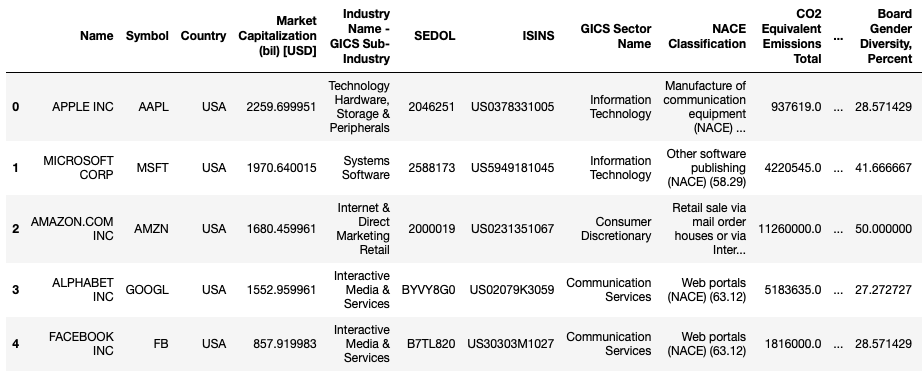
\includegraphics[scale=0.5]{dataset.png}
\caption{\textbf{Dataset excerpt}}
\label{fig:dataset}
\end{figure}
You will find the list of columns in Figure 3.
\begin{figure}[h!]
\centering
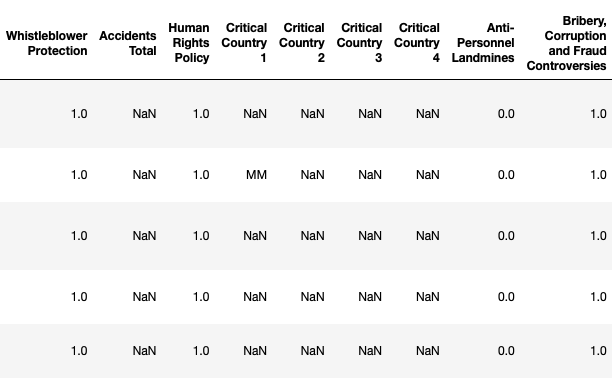
\includegraphics[scale=0.5]{dataset2.png}
\caption{\textbf{Dataset excerpt - 2}}
\label{fig:dataset2}
\end{figure}
 
\begin{figure}[h!]
\centering
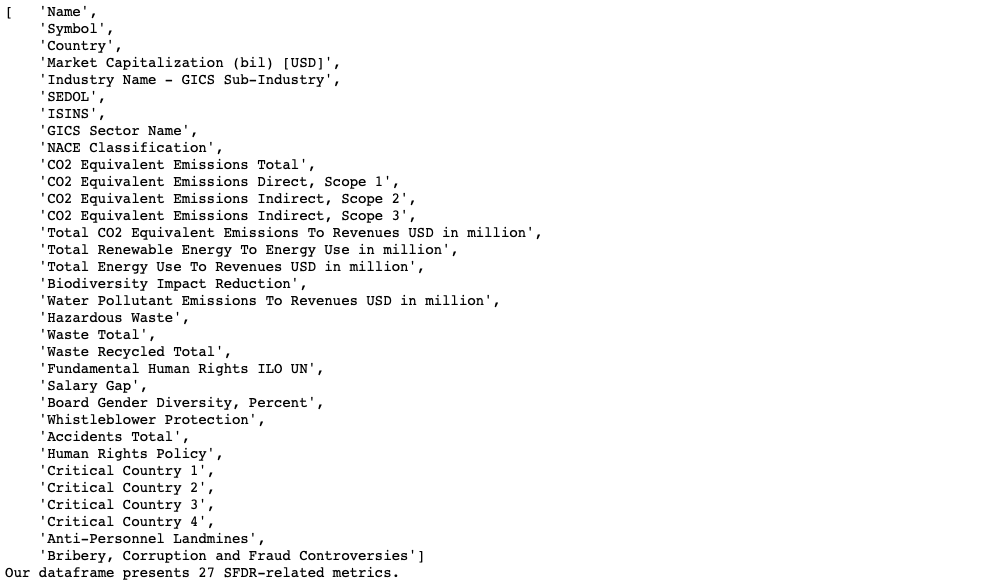
\includegraphics[scale=0.3]{columns.png}
\caption{\textbf{Column List}}
\label{fig:columns}
\end{figure}


Let us represent the input by a vector X of dimension \textbf{d = 69 features}\footnote{The GICS subsector was removed for encoding as it significantly complexified data dimensionality from 69 to over 200 features without improving classifier accuracy.} after binary encoding (28 columns before encoding). Except for the company's \textbf{Market Capitalization}, each feature corresponds to one of the \textbf{Sustainable Finance Disclosure Regulation mandatory disclosure metrics} or a proxy for it. After preprocessing, we are left with \textbf{n = 2,655 clean data inputs}.\newline
Our goal is to estimate $\mathbb{E}_\theta(Y \cdot|X)$, that is to say the theoretical expectancy of \textbf{Y our company's ESG class}, given \textbf{X its SFDR profile}. In other terms, suppose that each $(X_{i},Y_{i})$ couple,  company i and its ESG Class, are drawn from an underlying $(X,Y)$ distribution, which we are trying to estimate from the training set. This allows us to compare model performance efficiently.\newline
Y is defined as follows.
For \textbf{Thompson-Reuters}, the notation can take the following \textbf{twelve} values: A+, A, A-, B+, B, B-, C+, C, C-, D+, D, D-. For simplification purposes, we map each ESG grade to its corresponding letter. Our target Y can take the following \textbf{four} values: \textbf{A, B, C or D}, with A being the best possible class, and D the worst possible class.
For \textbf{MSCI}, the \textbf{nine} possible notations are: AAA, AA, A, BBB, BB, B, CCC, CC, C. We map each class to its first letter. We are then left with \textbf{three} values for target Y : \textbf{A, B and C}. Note that Thompson-Reuters and MSCI both adopt a \textbf{'best-in-class'} approach, meaning that they evaluate ESG performance at field level, whereas we cluster all companies together. Thus, non-supervised clustering can be said to resemble a \textbf{'best-in-universe'} approach.\newline



\subsubsection{Our approach consists of Feature Reduction, company clustering along SFDR metrics, and ESG Class Prediction.}

Our \textbf{approach} can be summarised as follows: 
\begin{itemize}
\item{Perform \textbf{feature reduction} to reduce data complexity from 69 to 20 features;}
\item{Use SFDR indicators to \textbf{cluster companies together} in an \textbf{unsupervised learning} setting}, and see whether companies are clustered by \textbf{industry} or not;
\item{Then, \textbf{predict ESG Scoring by either Thompson-Reuters or MSCI} in a \textbf{supervised learning setting, using SFDR indicators} as our features. Eventually, use the clusters to help us with the supervised learning task;}
\item{Ultimately, build a deep understanding of \textbf{ESG Performance predictors within SFDR indicators}, and \textbf{compare notation agency approaches}.} Indeed, we know from recent research that ESG Ratings do not converge \citep{notationdivergence}, which is a huge problem in the ESG industry. 
\end{itemize}
After manually \textbf{removing} the \textbf{GICS Subsector}\footnote{The industry a company belongs to as a granular level. For example, a company in the Financials sector could belong to the GICS Subsector of Financial Services. There are 158 sub-industries for 69 industries.} as a feature for simplification purposes and preprocessing our data, we select a limited number of features among the 69 original ones.\newline
\begin{enumerate}
    \item To this effect, we compare \textbf{Principal Component Analysis}, \textbf{Kernel Principal Component Analysis}, and \textbf{Random Forest selection} as feature reduction methods. The best feature reduction method, a \textbf{Random Forest}, was chosen by investigating how well the resulting features allowed to predict ESG Class. The features which presented the best accuracy were selected by using the top weights in a Random Forest algorithm\footnote{See details in section 0.4.2.} Thus, we keep \textbf{20 features} to predict Thompson-Reuters ESG Class.
    \item For \textbf{clustering}, we apply unsupervised methods to group companies together based on \textbf{SFDR-features, without integrating the final ESG Scoring}. Thus, we build our own understanding of ESG Performance. The best clustering method was mini-batch K-means\footnote{The best clustering method was defined as the one which, when clusters were used as a feature, led to the best Refinitiv ESG Score prediction}. The number of clusters was selected by elbow method adapted for a Cramer test \footnote{See section 0.4.5.3}.
    \item For our ESG Class prediction exercise, we benchmarked a \textbf{Logistic Regression}\footnote{see appendix for relevant equations}, a \textbf{K-Nearest-Neighbours} algorithm, and a \textbf{Random Forest} with little parameter tuning. We select the Random Forest Classifier algorithm as our best baseline model to build our ESG Scoring predictions, in a supervised learning setting. 
    \end{enumerate}


\subsection{Random Forests were our backbone algorithm.}

Random Forests are among the most popular \textbf{supervised learning} algorithms. They maintain high \textbf{accuracy} while being \textbf{scalable} with high data volumes\cite{scornet}. They are particularly efficient in cases where \textbf{data dimensionality} is high, especially when it exceeds the number of observations.
\subsubsection{Main principles: Ensembles with bootstrapping, Decision Trees (sequential splits with minimal impurity).}
The general framework is that of a \textbf{non-parametric classification estimation problem}. In this context, a Random Forest is an \textbf{ensemble} of \textbf{M decision trees}\footnote{M = 100 estimators is the default in sklearn}. In a classification setting, of the Random Forest \textbf{classifier} is the class predicted by \textbf{a majority of the M decision trees}:\newline 

\begin{gather*}
\overline{\hat{Y}} = \argmax_k f(k)
\end{gather*} where $f(k)$ is the count of the number of predictions for class k.

Each Decision Tree is built by randomly sampling the data in a principle called \textbf{bootstrapping}: for each estimator we want to build, we select a sub-sample of $N$ $(X_{i},Y_{i})$ couples within our dataset and train a classifier on it. 
Then, to predict y' based on X', we predict y' with each estimator.\newline
A given Decision Tree operates as follows. Through an \textbf{iterative process}, it  \textbf{partitions} the space \textbf{sequentially d times}, along each variable. The \textbf{optimal partition at each node} is found by minimising a previously defined criterion, often the \textbf{Gini}\footnote{We seek to minimise $\sum_{i}{p(i)*(1-p(i))}$, a measure of split impurity.} or the entropy criterion.\newline

\begin{figure}
\centering
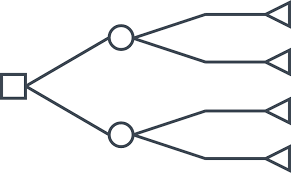
\includegraphics[scale=0.7]{decision_tree.png}
\caption{\textbf{Decision Tree Diagram}}
\label{fig:decisionTree}
\end{figure}


\subsubsection{Key parameters: Number of Estimators and Max depth.}
The main parameters to tune within a random forest are \textbf{the number of estimators}, and \textbf{k the tree depth}. Then, investigating the bootstrapping method and the minimum samples split is a good way to go.
Each parameter can be tuned keeping this rationale in mind: 
\begin{enumerate}
\item \textbf{M the number of trees in the forest}. Increasing M makes for more robust predictions as we aggregated over a higher number of estimators, but increases training time. In our case, there are not many datapoints so M can be high if needed. 
\item The \textbf{maximum depth} for each tree. The maximum number of decision levels in each tree. Deep trees tend to overfit the training set and generalise badly: that is, they have low bias and high variance.
\item The \textbf{minimum samples split}. The minimum number of data points placed in a node before the node is split. Playing with this hyperparameter allows to regularise individual Decision Trees, by avoiding splits on too few datapoints.
\item \textbf{Bootstrap method}. The way we sample data points to train our decision trees, with or without replacement. 
\end{enumerate}

\subsection{Data exploration confirms ESG data findings and gives us our first insights into ESG Performance.}
\subsubsection{Data collection process: we are missing some mandatory indicators altogether, like the Red List Species biodiversity impact.}

We gather \textbf{Sustainable Finance Discloure Regulation indicators}, as well as the \textbf{overall ESG Grade}, from \textbf{Thompson-Reuters} via their Refinitiv-Eikon platform. We first map each SFDR indicator to a Thompson-Reuters field, and extract a proxy for each metric when the field is not available (see Appendix).\newline


We are could not retrieve data on:  
\begin{enumerate}
\item \textbf{Biodiversity}: operations impact on red list species, and whether thheir operations are adjacent to biodiversity-rich sites;
\item \textbf{Deforestation} indicators;
\item \textbf{Water stress} and \textbf{untreated discharged waste water};
\item Whether the company implemented a \textbf{due diligence} on human rights and human trafficking;  
\item The \textbf{number of convictions for corruption}.
\end{enumerate}

For our benchmark on \textbf{MSCI ESG Grades}, we implement a scraping package for their open-source ESG-Corporate Tool\footnote{ESG Research Tool: https://www.msci.com/our-solutions/esg-investing/esg-ratings/esg-ratings-corporate-search-tool and Github repository: https://github.com/austinjhunt/msci\_esg} and gather data for each company in our dataset. 

\subsubsection{Geographical, industry and market capitalization bias.}

Let us first investigate three commonly mentioned biases in ESG : \textbf{industry} bias, \textbf{geographical} bias, and \textbf{market capitalization} bias.
We want to check two things:
\begin{enumerate}
    \item Whether \textbf{our dataset is biased} along those dimensions
    \item Whether \textbf{Thompson-Reuters and MSCI Scoring are influenced} by geography, industry, or market cap, although both scoring methodologies are \textbf{devised to neutralise} those biases.
\end{enumerate}
 
As is visible in Fig.5, our dataset is heavily biased towards the United-States. Generally speaking, we focus on European and American companies. Thus our whole enquiry focuses on Western companies and forgets about the emerging world. 

\begin{figure}[h!]
\centering
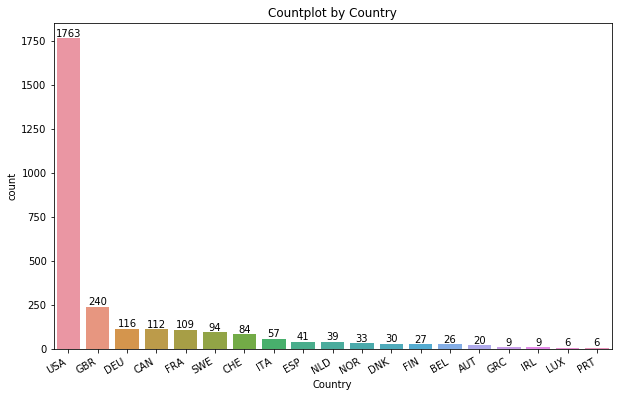
\includegraphics[scale=0.5]{country_distribution.png}
\caption{\textbf{Company country distribution count}}
\label{fig:countries}
\end{figure}

Regarding field distribution, all eleven GICS sectors are represented in our dataset as is visible in Fig.6 . However, Materials, Real Estate, Communication Services, Consumer Staples, Utilities and Energy are underrepresented versus Industrials, Financials, Consumer Discretionary, Information Technology and Health Care. 
\begin{figure}[h!]
\centering
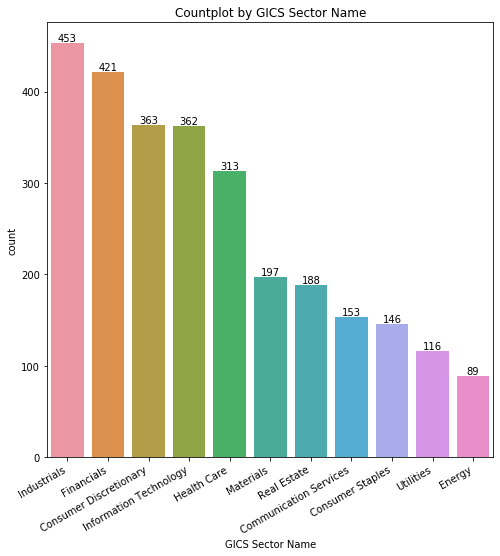
\includegraphics[scale=0.5]{sector_distribution.png}
\caption{\textbf{Company sector distribution count}}
\label{fig:sectors}
\end{figure}
 
We know from our expert interviews that some metrics do not compare the same at all across industries. Let us verify this assumption on CO$_{2}$ equivalent measures, carbon emissions by \$M turnover. 
\begin{figure}[ht]
\centering
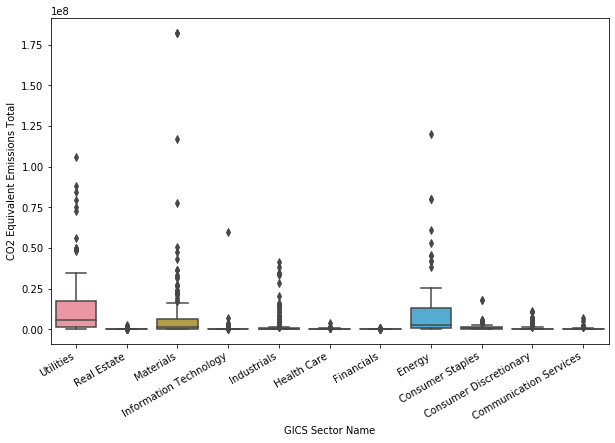
\includegraphics[scale=0.5]{CO2_equivalent_total_sector.png}
\caption{\textbf{Company sector CO$_{2}$ equivalent total}}
\label{fig:co2equivalent}
\end{figure}
In Figure 9, we see the boxplot of carbon intensity by Industry sector. As you can see, industry medians and spreads are significatly different - with a number of particularly high outliers in Utilities, Materials, Industrials and Energy. A one-way \textbf{ANOVA} on \textbf{CO2 Equivalent Emission means} by sector confirms that GICS industry strongly affects CO$_{2}$ emission means, with a p-value of order e-44, much lower than 0.05.  

\begin{figure}[h!]
\centering
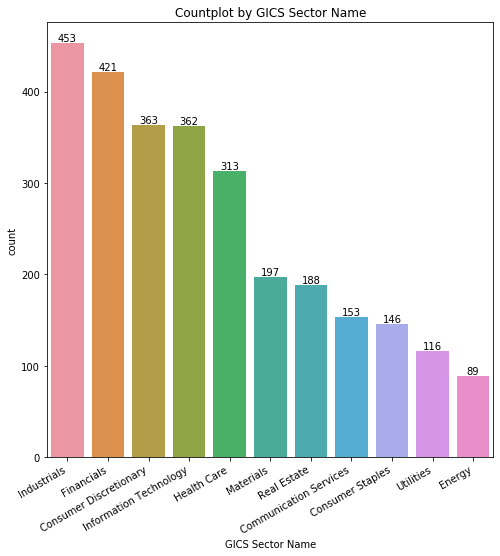
\includegraphics[scale=0.5]{sector_distribution.png}
\caption{\textbf{Market Capitalization Bias}}
\label{fig:marketcap}
\end{figure}
 
 
\subsubsection{Limited coverage on some indicators.}

We identify missing values within our SFDR metrics, as per Fig.11 and Fig. 12.
When a value is missing in Critical Country columns, it means that the company's operations don't take place in the critical country in question\footnote{As indicated in the Thompson-Reuters detailed methodology.}\newline
Thus, we are mostly missing data on \textbf{Water Pollutant emissions}. This is not surprising as Water Pollution is among \textbf{less well-covered environmental indicators} - carbon emissions take precedence. Noticeably, \textbf{Scope 3 carbon emissions} present a high missing value rate, which can be attributed to the fact that they are difficult to compute, report and compare given that they integrated indirect carbon emissions for which there is no standard calculation methodology. 
\begin{figure}[h!]
\begin{center}
\begin{tabular}{ |c|c|c| }
\hline
 Index & SFDR Metric & \% missing \\
 \hline\hline
 1 & Critical Country 1 & 99.9\% \\  
 2 & Critical Country 2 & 99.9\% \\
 3 & Critical Country 3 & 99.7\% \\
 4 & Critical Country 4 & 99.22\% \\
 5 & Water Pollutant Emissions To Revenues USD in Million & 96.8\% \\
 6 & Hazardous Waste & 76.7\% \\
 7 & Total Renewable Energy To Energy Use in million & 75.0\% \\
 8 & Accidents Total & 73.0\% \\
 9 & Waste Recycled Total & 72.1\% \\
 10 & CO2 Equivalent Emissions Indirect, Scope 3 & 68.6\% \\

\hline
\end{tabular}
\end{center}
\caption{\textbf{Top 10 categories by missing values}, \textit{percent}}
\label{fig:top10missing}
\end{figure}



\begin{figure}[h!]
\begin{center}
\begin{tabular}{ |c|c|c| }
\hline
 Index & SFDR Metric & \% missing \\
 \hline\hline
 1 & NACE Classification & 3.54\% \\  
 2 & Anti-Personnel Landmines & 5.81\% \\
 3 & Biodiversity Impact Reduction & 5.81\% \\
 4 & Fundamental Human Rights ILO UN & 5.81\% \\
 5 & Bribery, Corruption and Fraud Controversies & 5.85\% \\
 6 & Board Gender Diversity, Percent & 5.85\% \\
 7 & Whistleblower Protection & 12.41\% \\
 8 & CO2 Equivalent Emissions Total & 47.89\% \\
 9 & CO2 Equivalent Emissions Direct, Scope 1 & 51.93\% \\
 10 & CO2 Equivalent Emissions Indirect, Scope 2 & 52.27\% \\
\hline
\end{tabular}
\end{center}
\caption{\textbf{Bottom 10 categories by missing values}, \textit{percent}}
\label{fig:bottom10missing}
\end{figure}

\subsubsection{Feature Correlation.}
Let us observe SFDR feature correlation from Fig. 11.  
\begin{figure}[h!]
\centering
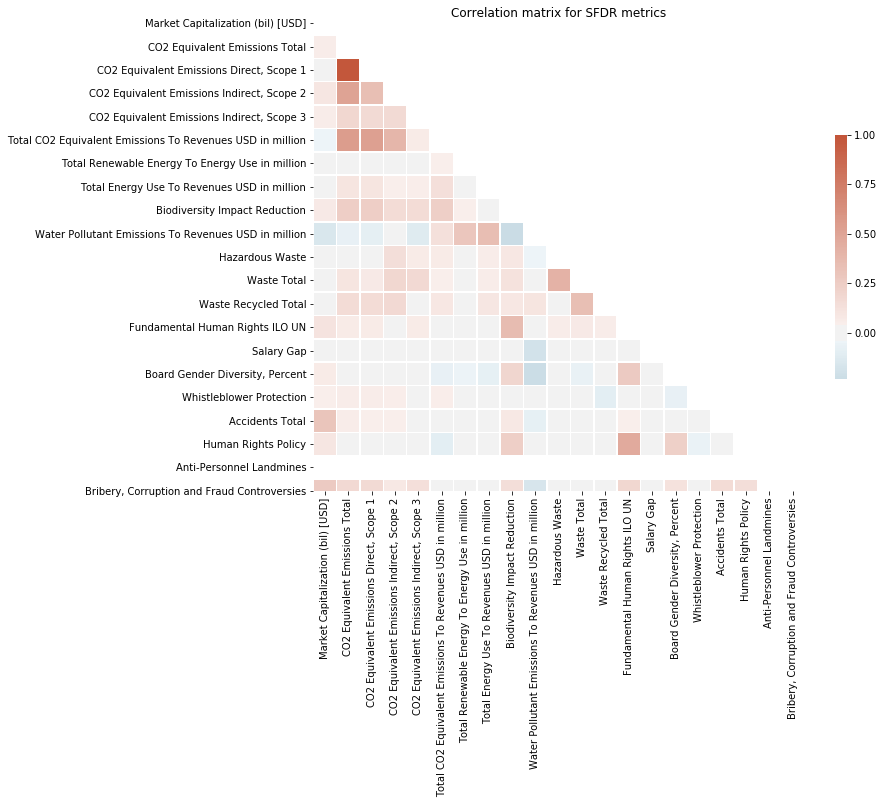
\includegraphics[scale=0.5]{correlation_matrix.png}
\caption{\textbf{SFDR Feature Correlation}}
\label{fig:correlation_sfdr}
\end{figure}

We can see that CO$_{2}$ emission variables are highly correlated in between themselves, especially direct emissions (scope 1 and 2) and with overall emissions. This goes well with what we would expect. 
It would seem that Water Pollutant Emission by turnover unit correlates negatively to market capitalization and the implementation of biodiversity impact reduction policies altogether. This is not surprising but bear in mind that we are missing over 95\% of all water pollutant data points, so we would have to crosscheck this result. 
Companies which implemented a Human Rights Policy usually signed the Fundamental ILO Human Rights Convention, which is not surprising either.

\subsection{Data pre-processing pipeline: filling with the industry median where relevant and conservative hypotheses on categorical variables.}

After data preprocessing, we are left with data for 2,655 observations.\newline
We know that environmental metrics especially, vary a lot from industry to industry.
To fill in missing values, we proceed in the following way :
\begin{itemize}
    \item We define continuous columns to use the industry median for, e.g. Total CO2 Emissions;
    \item We define categorical columns to fill conservatively, e.g. whether the company has implemented a Human Rights Policy or not;
    \item We define columns with too many missing values to keep , e.g. Water Pollutant Emissions to Revenues in USD.
\end{itemize}
Then, we drop the three rows with remaining missing values. 

\subsection{Clustering and Prediction}. 
We assume that the companies' \textbf{GICS subsector} presents redundant information with the overarching sector, and \textbf{remove the column}. This also highly simplifies our data without any effect on ESG Performance classification.\newline 
After One Hot Encoding, our data presents \textbf{high dimensionality} : \textbf{69 features} to process for our predictor. Keeping subsector information added over 150 features and did not a priori help predict ESG Scoring.\newline
We benchmark three methods to simplify our data : \textbf{Principal Component Analysis}, \textbf{Kernel Principal Component Analysis}, and \textbf{Feature Selection using a Random Forest}. To choose the best method, we \textbf{retro-adjust} by looking at \textbf{ESG Class prediction accuracy} on the test set with the resulting features. Using this metric, the best method was Random Forest Feature Selection. 

\subsubsection{Principal Component Analysis and Kernel Principal Components Analysis for dimensionality reduction show that our data is too complex to be lineary separable, but can be simplified using a kernel.}
Principal Component Analysis\footnote{See Appendix for detailed formalism} projects our data from a space of dimension d = 69 features into a space of a lower dimension d' by leveraging eigenvector decomposition of our matrix X (2651, 69) representing the input features. Principal Component Analysis assumes that the data can be expressed as a linear combination of X's eigenvectors \citep{pcatowardsdatascience}.
Each feature resulting from the Principal Component Analysis holds part of the information, or variance, present in our initial dataset. Thus, to determine d', we select a threshold of cumulated expressed variance we want our output features to hold. We select a threshold of 80\% cumulted explained variance, and let this determine d'.\newline

\begin{figure}[h!]
\centering
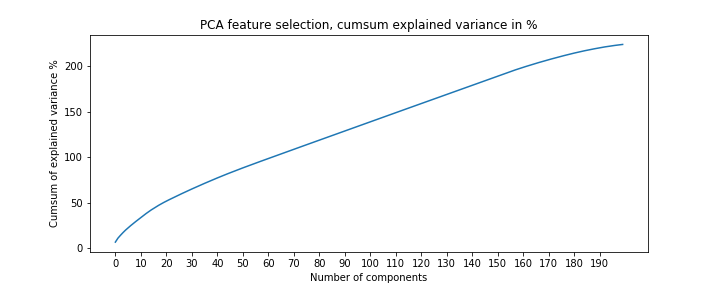
\includegraphics[scale=0.5]{PCA_feature_selection_cumsum.png}
\caption{\textbf{Explained variance as a function of the number of PCA features.}}
\label{fig:pcavariance}
\end{figure}

Now, note that PCA assumes that data is \textbf{linearly separable}. In our case, the data is too complex for this strong hypothesis to be verified, and PCA results are \textbf{sub-optimal}. As you can see in Figure 14, the cumulated sum of explained variance is nearly \textbf{linear}, meaning that each feature holds as much information as the others. If our feature reduction had worked well, we would see an elbow on the graph where adding an extra feature wouldn't add significantly more interesting information. Hence, the Principal Component transformation did not make any one feature significantly more useful than others. \newline

\begin{figure}[h!]
\centering
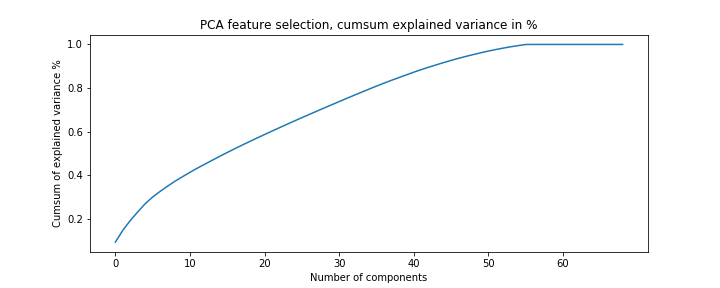
\includegraphics[scale=0.5]{PCA_feature_selection_cumsum_percent.png}
\caption{\textbf{Explained variance cumulated sum as a function of the number of PCA features.}, \textit{\%}}
\label{fig:pcavariancepercent}
\end{figure}

For PCA, you see that setting a threshold of 80\% leads to the selection of 34/69 features. Let us compare this to kernel PCA. 


Kernel PCA starts by applying a \textbf{non-linear transformation} to our data \textbf{before} performing a \textbf{Principal Components Analysis} on the result of this first step\citep{kernelpca}. Let us see if the cumulated variance graph yields more interesting results.\newline

\begin{figure}[h!]
\centering
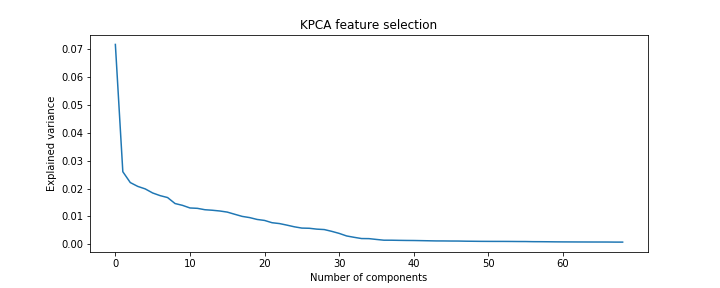
\includegraphics[scale=0.5]{KPCA_feature_selection.png}
\caption{\textbf{Explained variance as a function of the number of PCA features.}}
\label{fig:kpcavariance}
\end{figure}
From this graph, Kernel PCA works much better. Indeed, we clearly see that \textbf{some features hold significantly more information than others}. Let us check this using the cumulated variance graph in \%. 
\begin{figure}[h!]
\centering
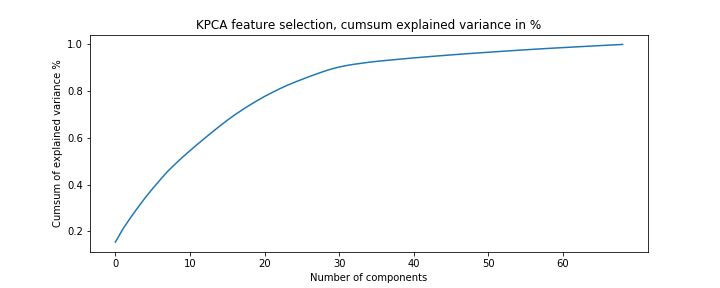
\includegraphics[scale=0.5]{KPCA_feature_selection_cumsum_percent.png}
\caption{\textbf{Explained variance cumulated sum as a function of the number of PCA features.}, \textit{\%}}
\label{fig:kpcavariancepercent}
\end{figure}

Here, we see an \textbf{asymptotic curve} starting at k=25 components. This means that \textbf{above 25 components or features}, adding an \textbf{extra feature} does not bring much more information to our data.

From Principal Component Analysis and Kernel Principal Component Analysis, we retain the following information:
\begin{enumerate}
    \item Our data is \textbf{too complex} to be \textbf{linearly separable};
    \item We are able to \textbf{summarise} it satisfactorily with approximately \textbf{25 features} explaining over \textbf{80\% variance}, provided that we apply a nonlinear kernel to our data before attempting to reduce it.
    \item However, to choose the best feature reduction method, we optimise by looking at \textbf{Thompson-Reuters ESG Class prediction accuracy on the test set}. Let us try a third method, \textbf{Random Forest selection}, to see how we want to transform our data. 
\end{enumerate}


\subsubsection{Random Forest for Feature Selection yielded the implementation of Fundamental Human Rights ILO UN convention and Market Capitalization as significant predictors.}
Feature importances are the weights a Random Forest attributes to different predictors when splitting the inputs into classes. Feature importance measures the \textbf{proportion of iterations where a variable was used to build a tree}. The \textbf{higher} the weight, the more \textbf{important a role} it played in the final \textbf{output prediction}. For this reason, looking at a Random Forest's feature importances is a good way to \textbf{prune} features when we have a lot. Note that here, unlike in PCA and KPCA, we are not transforming the features but simply selecting a subset of them. \newline 

\begin{figure}[h!]
\begin{center}
\begin{tabular}{ |c|c|c| }
\hline
 Index & Feature & Weight \\
 \hline\hline
 1 & Fundamental Human Rights ILO UN & 0.29 \\  
 2 & Human Rights Policy & 0.16 \\
 3 & Market Capitalization (bil) [USD] & 0.14 \\
 4 & Board Gender Diversity, Percent & 0.08 \\
 5 & Salary Gap & 0.03 \\
 6 & Hazardous Waste & 0.03 \\
 7 & Total Renewable Energy To Energy Use in million & 0.03 \\
 8 & CO2 Equivalent Emissions Indirect, Scope 2 & 0.02 \\
 9 & CO2 Equivalent Emissions Indirect, Scope 3 & 0.02 \\
 10 & Total CO2 Equivalent Emissions To Revenues USD in million & 0.02 \\
 11 & Accidents Total & 0.02 \\
 12 & CO2 Equivalent Emissions Direct, Scope 1 & 0.02 \\
 13 & Total Energy Use To Revenues USD in million & 0.02 \\
 14 & Biodiversity Impact Reduction & 0.02 \\
 15 & CO2 Equivalent Emissions Total & 0.02 \\
 16 & Waste Recycled Total & 0.02\\
 17 & Waste Total & 0.01 \\
 18 & Whistleblower Protection & 0.01 \\
 19 & x0\_USA & 0.01 \\
 20 & Bribery, Corruption and Fraud Controversies & 0.01 \\
\hline
\end{tabular}
\end{center}
\caption{\textbf{Features selected by Random Forest Regressor}, \textit{0.005 threshold}}
\label{fig:featureselection}
\end{figure}

Let us run a quick analysis on our output features. 
\begin{enumerate}
\setlength\itemsep{0em}
    \item The two most important features to predict Refinitiv ESG scoring are \textbf{governance-related} and concern the implementation of a \textbf{Human Rights Policy} within the organization. This is no surprise when we know that Governance is among the most standardised ESG measures within the sustainability field, and is well measured. It is also comparable in between industries, and since we are trying to predict ESG Scoring without accounting for industries, it is understandable that governance should take on more weight. 
    \item \textbf{Market Capitalization} comes third. This could point to a bias within the data towards capitalization. We know from our field investigation that some Asset Managers devise their own ESG scoring to circumvent capitalisation bias. Indeed, \textbf{bigger companies} have \textbf{more resources dedicated to transparency} and answering ESG notation agencies, inflating their ESG Scoring for that matter.
    \item We observe several occurrences of CO2 emissions as predictors: CO2 Equivalent Emissions as a total and by scope 1, 2 and 3, as well as CO2 intensity. It could be interesting to keep only one or two of these variables as they are correlated (see correlation matrix). 
    \item Some variables within our best predictors presented limited coverage : Hazardous Waste for example has 70\% missing values. They require specific attention to ensure that our missing value pre-processing did not bias the data. 
\end{enumerate}

Below, you can see how many companies in our dataset implemented the Fundamental Human Rights convention principles:

\begin{figure}[h!]
\centering
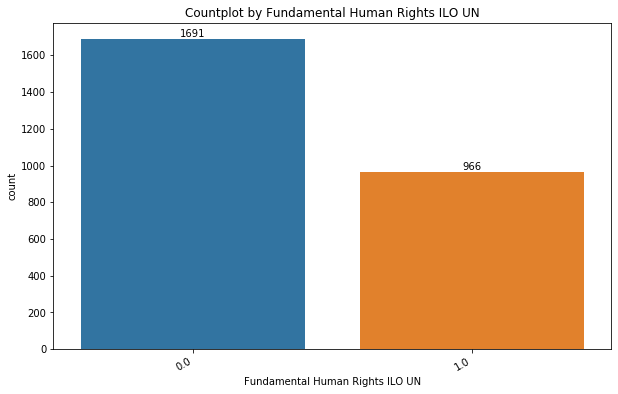
\includegraphics[scale=0.5]{human_rights.png}
\caption{\textbf{Fundamental Human Rights ILO UN count}}
\label{fig:human_rights}
\end{figure}

As you can see, 966 / 2 663 companies from our dataset (those we had these datapoints for) did implement the Fundamental Human Rights Convention, or approximately 36\% of them. This is lower than what one could expect, as the ILO convention is considered a basic Governance ESG measure. However, one could suppose that implementing the ILO rights convention thus means that the company performs better than average ESG-wise. Let us see if this is confirmed by a correlation matrix between the subset of 20 ESG metrics selected by our Random Forest and the ESG Scoring expressed as a 0-100 grade.

\begin{figure}[h!]
\centering
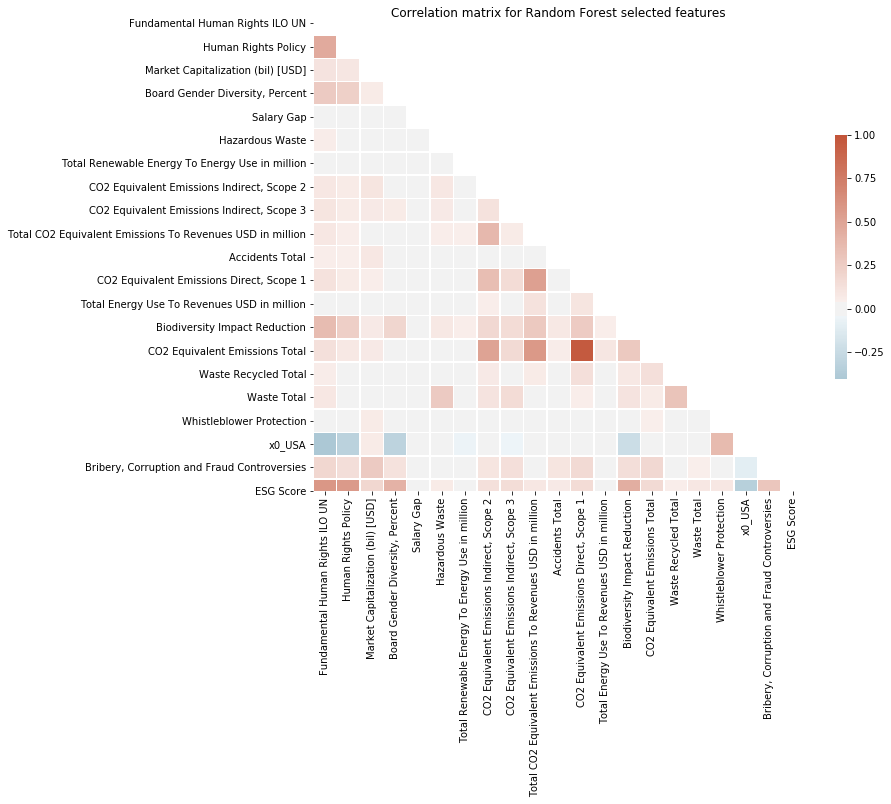
\includegraphics[scale=0.5]{corrplot_random_forest.png}
\caption{\textbf{Correlation matrix after feature selection, including target ESG Score Grade}}
\label{fig:rf_corrplot}
\end{figure}

Below, you will find a summary table of our results for all three feature reduction methods. 
\begin{figure}[h!]
\begin{center}
\begin{tabular}{ |c|c|c|c|c| }
\hline
 Index & Method  & Threshold & Number Features & Accuracy on Test (\%) \\
 \hline\hline
 1 & Principal Components Analysis & 80\% variance & 34/69 features & 50\% \\  
 2 & Kernel Principal Components Analysis & 80\% variance & 21/69 features & 50\%\\
 3 & Random Forest Feature Selection & 0.005 weight & 20/69 features & 50\%\\
\hline
\end{tabular}
\end{center}
\caption{\textbf{Dimensionality Reduction Results by method}}
\label{fig:dimensionality_benchmark}
\end{figure}


\subsubsection{The best clusters to separate ESG profiles without using the ESG class segmented companies along the implementation of Human Rights Policies, replicating our Random Forest feature selection findings.}

First, let us have a look at the overall ESG Class split for Thompson-Reuters on Fig.20. Class A represents 15\% of the dataset, B 39\%, C 35\%, and D 11\%. We will then compare this rating profile to the profile by cluster to see how well we managed to separate companies along ESG ratings, without using the ESG class information in the clustering.

\begin{figure}[h!]
\centering
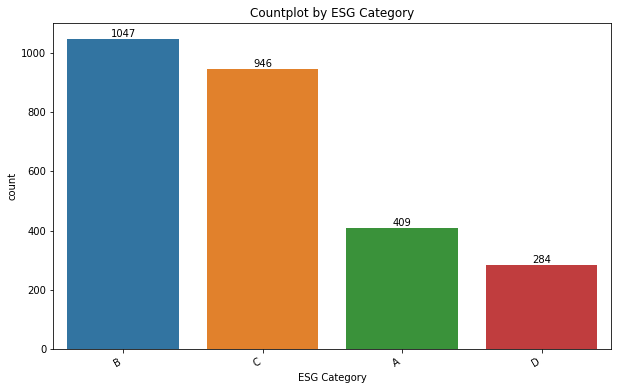
\includegraphics[scale=0.5]{ESG_score_distribution.png}
\caption{\textbf{ESG Class distribution}}
\label{fig:esgclass}
\end{figure}



We benchmark \textbf{ten clustering methods} on our dataset \citep{handbookclustering}, using only \textbf{Sustainable Finance Disclosure Regulation indicators} and the \textbf{Market Capitalization} as clustering features.\newline
Clustering occurs in an \textbf{unsupervised} manner, meaning that we do not manually tell our algorithm \textbf{what} the clusters are or how to do it across the features, but the algorithm finds it itself by \textbf{optimising along its clustering metric}. However, most algorithms still need an input such as the \textbf{number of clusters to define}.\newline
For instance, the \textbf{K-Means clustering algorithm} looks at each datapoint as a vector, and seeks to best \textbf{assign cluster centroids} so as to \textbf{maximise similarity between points in the same cluster} and \textbf{maximise dissimilarity between clusters}. Similarity is measured by looking at \textbf{Euclidean distance} in between vectors. The more similar two points are, the smaller their Euclidean distance.\newline
A challenge in clustering is that the measure of how well clustering is done depends on the user's \textbf{end goal}. In our case, we want the clusters to help discriminate in between ESG Classes.
Thus, post-clustering, we implement a Cramer's test in between the two following categorical variables: 
\begin{enumerate}
\setlength\itemsep{0em}
    \item The \textbf{cluster} that each company belongs to after applying the clustering algorithm
    \item The company's \textbf{ESG Class} according to Thompson-Reuters
\end{enumerate}
Note that since \textbf{ESG class was not used in the clustering process}, we are not \textbf{biasing} our clustering algorithm. We then use the resulting clusters as a feature within our Random Forest to backtest them, and select the clustering method which rendered the best accuracy on the test set.

To optimise the number of clusters for K-Means and Mini-Batch K-means, we implement an elbow method on a Cramer Test\footnote{The higher the value from the Cramer Test between two categorical variables, the more they are statistically related}, meaning that we observed how adding a cluster marginally increased the value of the Cramer test and looked for the number of clusters where the curve flattened.
Our two best clustering algorithms were \textbf{K-Means} and \textbf{Mini-Batch K-means}. We then finetuned the number of clusters for them and used them in our predictions. 

\begin{figure}[h!]
\centering
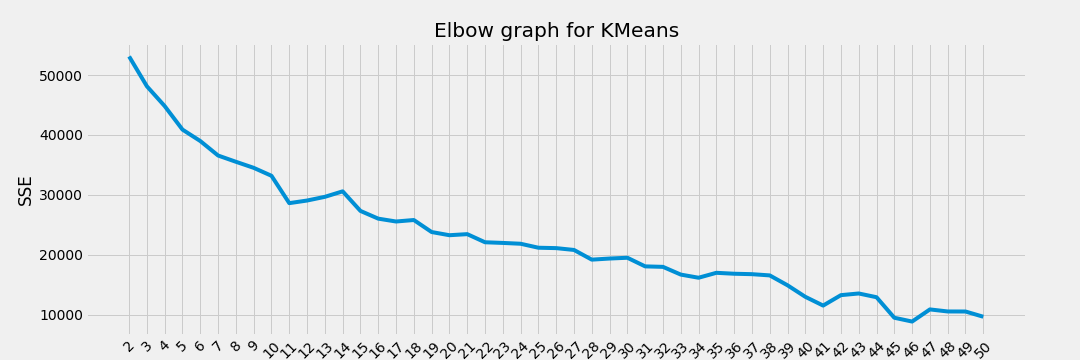
\includegraphics[scale=0.3]{elbow_graph_kmeans.png}
\caption{\textbf{Elbow Graph of Cramer's test as a function of the number of clusters}}
\label{fig:kmeans_elbow}
\end{figure}

With the K-Means algorithm, we achieve a Cramer Test value of 0.54 with just two clusters. When we visualise the ESG profiles of those clusters (Figure 22), we indeed managed to separate two groups: cluster 0 has significantly more D grades than the average, and cluster 1 has significantly more A grades than the overall dataset. However, we can see that B grades are present in a reasonable number in both groups. This means that our clustering \textbf{does not discriminate that well in between B companies}. 

\begin{figure}[h!]
\centering
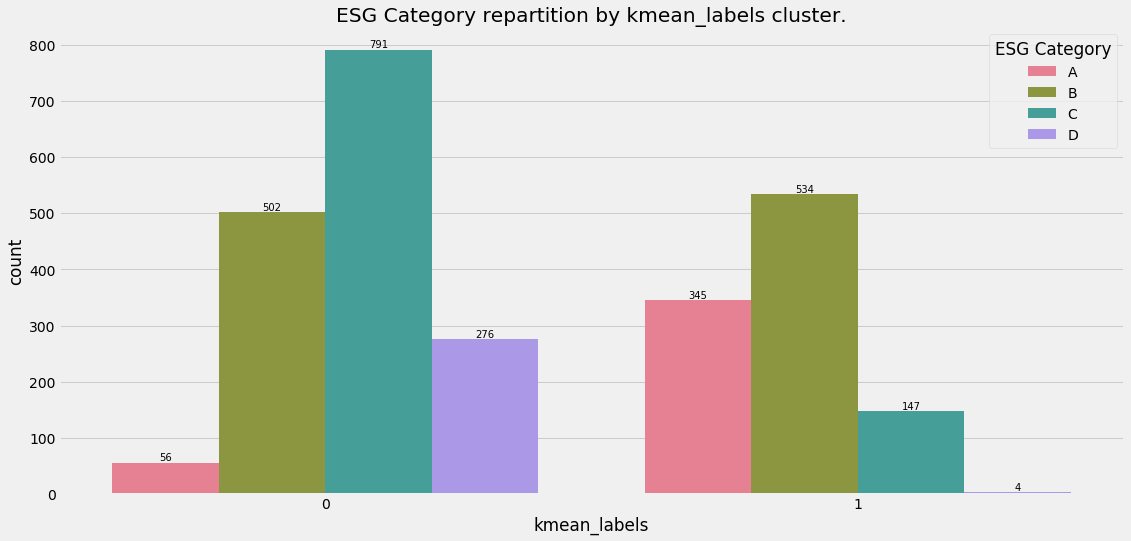
\includegraphics[scale=0.3]{ESG_cat_kmeans.png}
\caption{\textbf{ESG Category count by KMeans cluster}}
\label{fig:kmeans_esg}
\end{figure}

When we look at the split achieved using Mini-Batch K-means (Fig. 23), we can make a similar comments. Some clusters present significanlty more A profiles, other more D profiles. However, B profiles are present everywhere, meaning that our clustering fails to isolate B grades from other companies.

\begin{figure}[h!]
\centering
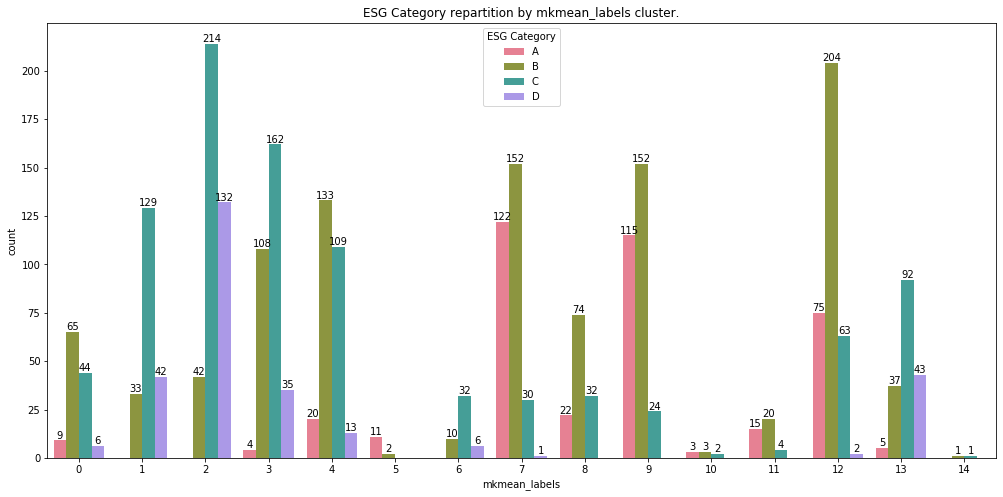
\includegraphics[scale=0.3]{ESG_cat_mkmeans.png}
\caption{\textbf{ESG Category count by Mini-Batch K-Means cluster}, }
\label{fig:mkmeans_esg}
\end{figure}

\subsubsection{Predictions: Using the clusters to segment our data, we achieve 58\% accuracy with cross-validated Random Forests for four classes.}
In this section, we now aim to predict the class an observation, alias a company, will be assigned by Thompson-Reuters.\newline
As stated in our introductory context section, we decide to simplify our categories by only keeping the letter from the score. For example, A++ becomes A and C- becomes C. We are left with \textbf{four classes}: A, B, C and D.\newline
Below, you can 
\begin{figure}[h!]
\begin{center}
\begin{tabular}{ |c|c|c|c| }
\hline
 Index & Algorithm & Parameters & Accuracy \\
 \hline\hline
 1 & Random Forest & 200 estimators & 56.87\% \\  
 2 & Logistic Regression & penalty: l1 & 54.05\% \\
 3 & KNN & 15 neighbours & 52.92\% \\
\hline
\end{tabular}
\end{center}
\caption{\textbf{Algorithm Benchmark with sklearn default parameters}, \textit{limited tweaking}}
\label{fig:benchmark}
\end{figure}

Using sklearn default parameters, we can see that the overall accuracy of the Random Forest is the best (Figure 24). Let us see if we can say more by looking at the accuracy breakdown by class.

\begin{figure}[h!]
\centering
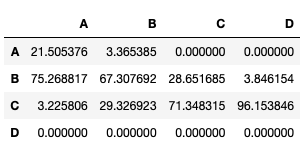
\includegraphics[scale=0.7]{logreg_benchmark.png}
\caption{\textbf{Logistic Regression Accuracy by Class}, \textit{percent}}
\label{fig:logreg_benchmark}
\end{figure}

Logistic regression massively predicts A-class as a B (75\%) and D-class as a C (96\%), while predicting B and C class rather well (67\% and 71\% accuracy respectively). From class imbalance, we know that an algorithm which always predicted B would have 39\% accuracy (Class A represents 15\% of the dataset, B 39\%, C 35\%, and D 11\%). So, we must not be satisfied with such results.

\begin{figure}[h!]
\centering
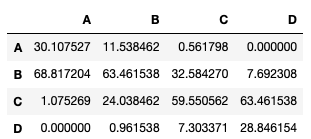
\includegraphics[scale=0.7]{knn_benchmark.png}
\caption{\textbf{{K-Nearest-Neighbours Accuracy by Class}}, \textit{percent}}
\label{fig:knn_benchmark}
\end{figure}

To a lesser extent, the same consideration applies to our KNN algorithm. Indeed, it often predicts class A as B, and C as B. 

\begin{figure}[h!]
\centering
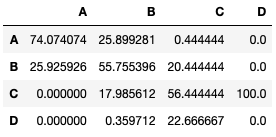
\includegraphics[scale=0.7]{rf_benchmark.png}
\caption{\textbf{{Random Forest Accuracy by Class}}, \textit{percent}}
\label{fig:rf_benchmark}
\end{figure}

Now looking at the Random Forest accuracy by class, it is clear that this model is the best one : indeed, it predicts 75\% of A classes accurately! Moreoever, we can assume that detecting extreme grades better is more important if we are either trying to hedge ESG risk or identify ESG opportunities. Note that the error on class D is actually one mistake, since we had only one D class in the test set. 

\begin{figure}[h!]
\centering
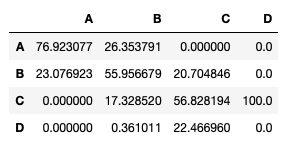
\includegraphics[scale=0.7]{rule_benchmark.png}
\caption{\textbf{{Rule-Based Random Forest Accuracy by Class}}, \textit{percent}}
\label{fig:rule_benchmark}
\end{figure}

Now if we check the performance of our rule-based random forest model on each class (Figure 28), trained specifically on some of the clusters we devised with mkmeans, we see that we slightly improved our predictions on A, B and C classes, meaning that we could explore this solution further if we wanted to yield significantly better accuracy.


\begin{figure}[h!]
\begin{center}
\begin{tabular}{ |c|c|c|c| }
\hline
 Index & Algorithm & Parameters & Accuracy \\
 \hline\hline
 1 & Custom Random Forest & 200 estimators & 57.25\% \\  
 2 & Random Forest with KMean labels & 200 estimators & 55.93\% \\
 3 & Random Forest with Mini-Batch KMean labels & 200 estimators & 55.93\% \\
\hline
\end{tabular}
\end{center}
\caption{\textbf{Algorithm Benchmark with sklearn default parameters}, \textit{limited tweaking}}
\label{fig:endbenchmark}
\end{figure}
Finally, on Fig. 29 you see our conclusion: our best performing algorithm overall is our custom random forest, which we trained specifically on some of the mkmeans clusters we created during the unsupervised learning phase. 

\subsection{Cross-Validation}
Given that our best performing model is a Random Forest, we finetune it using cross-validation. To this effect, we leverage the GridSearch CV module in sklearn. 

Below, you will find the parameter grids. 

\begin{figure}[h!]
\begin{center}
\begin{tabular}{ |c|c|c|c| }
\hline
 Index & Parameter & Values & Selected Value \\
 \hline\hline
 1 & Number of estimators & [100,200,300,400,500] & 400 \\  
 2 & Max depth & [5,10,15,20] & 5 \\
 3 & Min samples split & [2,5,10,20] & 20 \\
 4 & Max features & ["auto", "sqrt", "log2"] & log2 \\
 4 & Class Weight & [None, "balanced"] & None \\
 
\hline
\end{tabular}
\end{center}
\caption{\textbf{Parameter Grids for Cross-Validation}, \textit{Random Forest}}
\label{fig:crossval}
\end{figure}
As you can see in Fig. 31, finetuning our baseline Random Forest improved its overall accuracy by 1\%. 
For the rule-based random forest, we keep the same best parameters and our accuracy reaches XX\%. 
\begin{figure}[h!]
\begin{center}
\begin{tabular}{ |c|c|c| }
\hline
 Index & Algorithm &  Accuracy \\
 \hline\hline
 1 & Best Parameters Random Forest & 57.82\% \\
 3 & Best hyperparameters Rule-based Random Forest & XX\% \\
\hline
\end{tabular}
\end{center}
\caption{\textbf{Algorithm Benchmark with sklearn default parameters}, \textit{limited tweaking}}
\label{fig:bestbenchmark}
\end{figure}


\subsection{Results Discussion}
\subsubsection{Model performance was good and predicted extreme classes well.}
Our final accuracy of \textbf{58\%} to discriminate between \textbf{four unbalanced classes} is good.\newline
Indeed, if we had \textbf{two balanced classes} and guessed at \textbf{random}, we would have \textbf{50\% accuracy}. In our case, training with \textbf{four unbalanced} classes, we are right \textbf{six times out of ten} and with a \textbf{simple} yet \textbf{robust} algorithm.\newline
Additionally, unlike \textbf{Logistic Regression} and \textbf{K-Nearest Neighbours}, our Random Forest performs very well on \textbf{extreme} classes. It mostly predicts A and D correctly, when Logistic Regression predicted B and C most of the time\footnote{Given the classes were unbalanced, it look like it had good accuracy when it reality it did poorly.}. Moreover, when our Random Forest predicts a Thompson-Reuters class wrongly, it predicts the closest class.\newline

\subsubsection{Model interpretation teaches us some more about ESG Performance.}

\subsubsection{There is still a lot to be explored to improve accuracy}
\begin{enumerate}
    \item We could have reduced feature \textbf{dimensionality} with an \textbf{auto-encoder};
    \item We could have \textbf{normalised} by \textbf{field} and \textbf{geography};
    \item We could have trained custom random forests using the \textbf{Human Rights Policy Boolean} to split our dataset
    \item We could have explored \textbf{B and C} classes more to differentiate in between them
    \item We could have trained \textbf{one model per sector} or \textbf{one model per geography} to see if it made any difference
    \item We could have devised a method to select the clusters to train upon mathematically rather than entering them manually
\end{enumerate}
\begin{titlepage}
\section{Conclusion}
In this Master Thesis, we explored the intricacies of ESG Data and the potential for \textbf{emerging frameworks} to become the baseline for ESG Analysis.\newline
With the rise of \textbf{environmental} concerns, \textbf{climate risk} at their forefront, Sustainable Finance and ESG are becoming commonplace - some would say \textbf{mainstream}. This makes for heightened risks of \textbf{financial greenwashing}, but also signals a \textbf{ profound market shift} with regulators doubling down on the matter. The European Union is \textbf{changing gear} to make corporate extra-financial performance comparable for investors and civil society by offering  \textbf{standardised} - yet \textbf{imperfect} - frameworks, in a context where data is \textbf{collected}, \textbf{pre-processed} and \textbf{analysed} mostly by \textbf{American-owned notation agencies}, making ESG a \textbf{geopolitical} concern.\newline
Several question marks remain however. Before thinking to disclosure, how can companies of \textbf{all sizes} \textbf{track} their extra-financial data in the best possible way? How can ESG data be made \textbf{relevant to investment decisions} and financial returns, without losing its \textbf{ethical} purpose? Will \textbf{social matters}, like environmental issues today, become the next hot topic? Does it make sense to \textbf{scale} ESG Data capabilities, or can a rigorous analysis only occur on a \textbf{case by case} basis given company heterogeneity by geography, industry, and market capitalisation? This is what impact advocates would tend to say.\newline
Our own ESG analysis confirmed that :
\begin{enumerate}
    \item Notation Agency ratings \textbf{do not converge}, even on a pool of \textbf{well documented} Western world companies;
    \item When grouping companies using a \textbf{'best-in-universe'} approach, that is to say without normalising by industry or geography, Governance indicators and notably Human Rights Policies become important \textbf{clustering} variables and \textbf{ESG Class} predictors;
    \item Sustainable Finance Disclosure Regulation indicators are difficult to obtain at \textbf{portfolio level}.
\end{enumerate}

So, \textbf{what does ESG data teach us about corporate sustainability}?\newline
First, that there is \textbf{no common definition} of what a sustainable company is - be it for \textbf{companies themselves}, \textbf{investors}, or \textbf{civil society}. For instance, \textbf{'best-in-class'} ratings, where a companies' sustainability is evaluated versus its peers, makes sense from a financial point of view if we do not want to restrict the investment universe, but is usually met with incomprehension by end consumers: \textit{why do I have Total in my green portfolio}?. It then comes as \textbf{no surprise} then that \textbf{notation agency ESG ratings} should \textbf{diverge} since they \textbf{aggregate} many factors in one single signal - environmental, social, governance matters mingling over 150 sub-indicators, in different industries and geographies, for vastly different capitalizations.\newline
And European ESAP data hubs offer no guarantee of \textbf{framework} harmonisation. Indeed it seems that the more clout ESG gains, the more \textbf{hyper-specialised} data providers are needed. This means that harmonisation could be happening at a \textbf{sub-indicator} level, in terms of measuring methodology, as it is starting to happen for carbon emission tracking.\newline
Although encouraging company disclosure is paramount a \textbf{stepping stone} towards ESG evaluation, it will not be enough. True value is to be found in the \textbf{analysis} that will be made of the data, and the spirit in which it is done. 
\end{titlepage}

\bibliography{references}


\section{Appendix}

\begin{figure}[h!]
\begin{center}
\begin{tabular}{|c|c|c|}
\hline
 Index & Field & Framework\\ 
\hline\hline
 1 & Anti-personnel mines and cluster bombs & Ottawa and Oslo Treaties\\  
\hline
 2 & Chemical, biological, and depleted uranium weapons & None\\
\hline
 3 & UN Global Compact violation & UN Global Compact 10 principles\\
\hline
 4 & Coal & Ethical\\
\hline
 5 & Tobacco & Ethical\\
\hline
\end{tabular}
\end{center}
\label{fig:amundiexample}
\caption{\textbf{Amundi ESG Exclusions 2020 example}\cite{amundi}}
\end{figure}

\begin{center}
\begin{tabular}{ c c c }
 cell1 & cell2 & cell3 \\ 
 cell4 & cell5 & cell6 \\  
 cell7 & cell8 & cell9 
\end{tabular}
\end{center}
\label{fig:sfdrindicators}

\begin{figure}[h!]

\centering
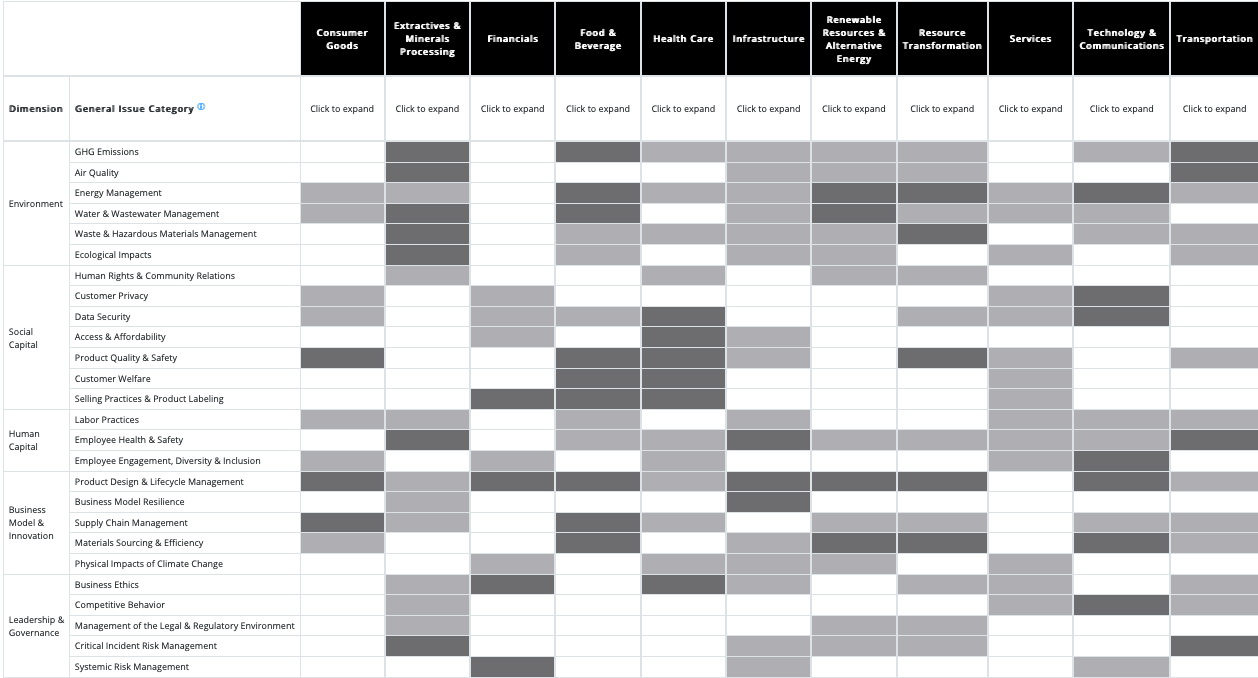
\includegraphics[scale=0.2]{materiality_map.png}
\caption{\textbf{SASB Materiality Map}, \textit{material issues by industry}}
\label{fig:materialitymap}
\end{figure}


\begin{figure}[h!]
\begin{center}
\begin{tabular}{ |c|c|c|c| }
\hline
 Index & Cluster Method & Rule Model Accuracy & Optimal Parameter\footnote{If we selected the method for cluster finetuning.} \\
 \hline\hline
 1 & KMeans & 53.30\% & 2 clusters \\  
 2 & Mini-Batch KMeans & 53.3\% & 15 clusters \\
 3 & Affinity & Too many labels & N/A \\
 4 & DBSCAN & 47.83\% & N/A \\
 5 & BIRCH & 54.99\% & N/A \\
 6 & Gaussian Mixture & 52.54\% & N/A \\
 7 & Spectral Clustering & Too few samples per cluster & N/A \\
 8 & Aggregation & 55.56\% & N/A \\
 9 & Mean Shift & Too few samples per cluster & N/A \\
 10 & Optics & 53.48\% & N/A \\
\hline
\end{tabular}
\end{center}
\caption{\textbf{Clustering Methods Benchmark}, \textit{0.005 threshold}}
\label{fig:clustering_benchmark}
\end{figure}


\begin{figure}
    \centering
As a reminder, here is the important equation for logistic regression:
\begin{enumerate}
    \item Logistic Regression:  \begin{multline} 
{P}_\theta(Y|X) = \frac{\exp(-\sum_{i}{\beta_{i}X_{i}})}{1 + \exp(-\sum_{i}{\beta_{i}X_{i}}}) \label{eq:glm1} 
\end{multline}
\end{enumerate}
    \label{fig:logreg}
    \caption{Logistic Regression equation}
\end{figure}

\end{document}